\documentclass[10pt,a4paper]{article}

% ------------------------------------------------------------------
% Assignment #3 - Anonymization of a Dataset with Risk and Utility
% Adult dataset (UCI) - ARX 3.9.2
% ------------------------------------------------------------------
\usepackage[utf8]{inputenc}
\usepackage[T1]{fontenc}
\usepackage[a4paper,margin=2.1cm]{geometry}
\usepackage{graphicx}
\usepackage{booktabs}
\usepackage{array}
\usepackage{amsmath}
\usepackage{amssymb}
\usepackage{xcolor}
\usepackage{caption}
\usepackage{subcaption}
\usepackage{enumitem}
\usepackage{pgfplots}
\pgfplotsset{compat=1.18}
\usepackage[hidelinks]{hyperref}
\usepackage{titlesec}

% compact spacing
\titlespacing*{\section}{0pt}{6pt}{3pt}
\titlespacing*{\subsection}{0pt}{4pt}{2pt}
\setlist{nosep,leftmargin=1.3em}
\captionsetup{font=small,labelfont=bf}
\renewcommand{\arraystretch}{1.05}
\setlength{\parskip}{2pt}
\setlength{\parindent}{0pt}

\newcommand{\leqK}{\(\leq\)50K}
\newcommand{\gtK}{\(>\)50K}

\title{%
    \textbf{Assignment \#3: Anonymization of the \textit{Adult Dataset} with Risk and Utility Analysis} \\[0.5em]
    \large Security and Privacy --- FCUP 2025/2026
}
\author{
    Francisco Machado (up202403514) \and
    Rodrigo Dias (up202407281)
}


\begin{document}
\maketitle
\vspace{-0.8cm}

% ==================================================================
\section{Introduction}
% ==================================================================
This work performs the anonymization of the \textit{Adult dataset} (Census Income, UCI), comprising
\textbf{32{,}561 records} and 15 attributes, using the ARX 3.9.2 tool. The goal is to classify the attributes
according to their role in privacy, characterize the re-identification risk of the original dataset, apply two
privacy models (\textit{k}-anonymity and \textit{k}-anonymity\,+\,$\ell$-diversity), and analyze the trade-off
between risk and utility as a function of the privacy models' parameters.

% ==================================================================
\section{Attribute Classification}
% ==================================================================
Classification was based on the \textbf{distinction} metric (percentage of distinct values, closeness to a
key) and \textbf{separation} (percentage of record pairs the attribute can distinguish), as analyzed in ARX's
\textit{Quasi-identifiers} tab. Table~\ref{tab:class} summarizes the values and the assigned classification.

\begin{table}[h]
\centering\footnotesize
\begin{tabular}{l r r l p{6.6cm}}
\toprule
\textbf{Attribute} & \textbf{Dist.\%} & \textbf{Sep.\%} & \textbf{Class} & \textbf{Justification} \\
\midrule
fnlwgt          & 66{,}48 & 99{,}99 & Identifying & Near-unique distinction; sampling weight with no analytical value. \\
education-num   & 0{,}05  & 80{,}96 & Identifying & Exact numeric duplicate of \textit{education} - removed to avoid duplicating the dimension. \\
age             & 0{,}22  & 97{,}87 & QID & Very high separation; age is known/inferable and highly discriminative. \\
occupation      & 0{,}05  & 90{,}29 & QID & High separation; often public (e.g.\ LinkedIn). \\
education       & 0{,}05  & 80{,}96 & QID & Known demographic, high separation. \\
hours-per-week  & 0{,}29  & 76{,}25 & QID & Observable/inferable, high separation. \\
marital-status  & 0{,}02  & 66{,}01 & QID & Public demographic; contributes to the identifying combination. \\
workclass       & 0{,}03  & 49{,}71 & QID & Observable demographic. \\
sex             & 0{,}01  & 44{,}28 & QID & Publicly known; a multiplier within the combination. \\
race            & 0{,}02  & 25{,}98 & QID & Visible/known demographic attribute. \\
native-country  & 0{,}13  & 19{,}66 & QID & Low separation (90\% US), but rare values make individuals unique. \\
income          & 0{,}01  & 36{,}57 & Sensitive & Target attribute, financially sensitive; protected via $\ell$-diversity. \\
capital-gain    & 0{,}37  & 15{,}93 & Sensitive & Private financial data to protect against inference. \\
capital-loss    & 0{,}28  & 9{,}10  & Sensitive & Idem: private financial information. \\
relationship    & 0{,}02  & 73{,}21 & Insensitive & Redundant with \textit{marital-status}/\textit{sex}; kept without transformation. \\
\bottomrule
\end{tabular}
\caption{Classification of the 15 attributes based on distinction and separation.}
\label{tab:class}
\end{table}

 \begin{figure}[h]
  \centering
  \includegraphics[width=\textwidth]{image.png}
  \caption{ARX \textit{Quasi-identifiers} tab showing the distinction and separation
  values used to classify the attributes (cf. Table~\ref{tab:class}).}
  \label{fig:qid}
  \end{figure}

\textbf{Justification notes.} (i) \textit{fnlwgt} and \textit{education-num} are both \textit{Identifying} but for
different reasons: the former due to near-unique distinction (66\%), the latter because it is an exact copy of
\textit{education} (avoids counting the same dimension twice among the QIDs). (ii) \textit{income} is
\textit{Sensitive} rather than a QID because it is the target of inference: protecting it is the goal of
$\ell$-diversity; being \textbf{binary} (\leqK\ / \gtK), it limits the maximum value of $\ell$ to~2.
(iii) \textit{relationship} is \textit{Insensitive} as it correlates strongly with \textit{marital-status} and
\textit{sex}: classifying it as a QID would add redundancy with no privacy gain.

\textbf{Risk arises from the combination.} No single QID identifies an individual, but the combination of the
9 QIDs produces \textbf{26{,}536 equivalence classes}, of which \textbf{23{,}512 are unique records (72{,}21\%)}.
The combined distinction is 81{,}5\%. It is this exposure that motivates the anonymization.

% ==================================================================
\section{Coding Models: Generalization Hierarchies}
% ==================================================================
A generalization hierarchy was defined for each QID. Numeric attributes used \textbf{interval}-based
hierarchies; categorical ones were built by successively grouping values (\textit{merge}).
Table~\ref{tab:hier} summarizes the structure.

\begin{table}[h]
\centering\footnotesize
\begin{tabular}{l l c p{8.0cm}}
\toprule
\textbf{QID} & \textbf{Type} & \textbf{Levels} & \textbf{Structure (from base level to top)} \\
\midrule
age            & Intervals & 5 & exact $\to$ 5 years $\to$ 10 years $\to$ 20 years $\to$ \texttt{*} \\
hours-per-week & Intervals & 4 & exact $\to$ blocks of 10 $\to$ 2 bands (part/full-time) $\to$ \texttt{*} \\
education      & Categorical & 4 & 16 values $\to$ \{Without-HS, HS, Higher-Ed, Post-Grad\} $\to$ \{Basic, Advanced\} $\to$ \texttt{*} \\
marital-status & Categorical & 4 & 7 values $\to$ \{Married, Was-married, Single\} $\to$ \{Has-been-married, Single\} $\to$ \texttt{*} \\
workclass      & Categorical & 3 & 8 values+\texttt{?} $\to$ \{Government, Self-emp, Private, Unemployed\} $\to$ \texttt{*} \\
occupation     & Categorical & 3 & 14 values+\texttt{?} $\to$ \{White-collar, Blue-collar, Service, Other\} $\to$ \texttt{*} \\
race           & Categorical & 3 & 5 values $\to$ \{White, Non-White\} $\to$ \texttt{*} \\
sex            & Categorical & 2 & \{Male, Female\} $\to$ \texttt{*} \\
native-country & Categorical & 3 & 41 values+\texttt{?} $\to$ continents $\to$ \texttt{*} \\
\bottomrule
\end{tabular}
\caption{Generalization hierarchies defined for the 9 quasi-identifiers.}
\label{tab:hier}
\end{table}

\textbf{Relevant grouping decisions.}
\begin{itemize}
\item \textbf{age vs hours-per-week.} Interval width does not follow a formula: for \textit{age}, with a spread
distribution, fine 5-year intervals preserve useful information (age bands are analytically meaningful),
justifying a deep hierarchy. For \textit{hours-per-week}, where \textbf{46{,}7\% of records are exactly 40h} and
56{,}3\% fall in the 40--49h block, 5h blocks would be redundant; blocks of 10h were used, sufficient to
distinguish part-time / full-time / overtime.
\item \textbf{Dominant categories stay isolated.} In \textit{race}, \textit{White} (85{,}4\%) and in
\textit{native-country}, \textit{United-States} ($\sim$90\%) are so common that they carry no risk; the
\emph{rare} categories (those that make individuals unique) are generalized instead. It is acknowledged as
a \textbf{limitation} that grouping ethnic minorities into a single \textit{Non-White} erases distinctions
between groups: a pragmatic anonymization choice, acceptable given the objective.
\item \textbf{Disambiguation of \textit{native-country}.} The value \texttt{South} is not explicitly documented;
we follow the common interpretation that it corresponds to \emph{South Korea} and grouped it under Asia. This
decision is supported by the data itself: \textbf{96{,}2\% of records with \texttt{South} have race
Asian-Pac-Islander}, a proportion consistent with (and higher than) that of the confirmed Asian countries. By
the same truncation logic, \texttt{Hong} was treated as \emph{Hong Kong} (Asia). Missing values (\texttt{?})
were mapped directly to \texttt{*}.
\end{itemize}

% ==================================================================
\section{Risk of the Original Dataset}
% ==================================================================
The risk analysis (\textit{prosecutor} model, the most conservative attack) confirms the high exposure of the
original dataset: a \textbf{maximum risk of 100\%} (unique records re-identifiable with certainty) and an
\textbf{average risk of 81{,}5\%}. About \textbf{72{,}2\%} of records are \textit{sample uniques} and the
percentage of \textit{population uniques} (PITMAN model) is 13{,}9\%. The average equivalence-class size is only
1{,}23 records. These values constitute the \textbf{baseline} for assessing the effect of anonymization.

% ==================================================================
\section{Privacy Models: Risk and Utility}
% ==================================================================
Two models were applied with \textbf{global transformation} and a \textbf{suppression limit of 100\%}, using
\textit{Loss} as the utility metric (geometric mean, generalization/suppression factor = 0{,}5). Information
loss is reported by the \textit{Score} of the optimal solution (0 = no loss, 1 = total loss).

\subsection{Model 1: \textit{k}-anonymity}
We varied $k \in \{2,5,10,25,50,100\}$. Table~\ref{tab:m1} presents the results and Figure~\ref{fig:plots} the
risk and utility plots as a function of $k$.

\begin{table}[h]
\centering\footnotesize
\begin{tabular}{c c c c c c}
\toprule
$k$ & \textbf{Max.\ risk (\%)} & \textbf{Success rate (\%)} & \textbf{Avg.\ class size} & \textbf{Suppression (\%)} & \textbf{Loss (Score)} \\
\midrule
2   & 50{,}0  & 7{,}47 & 13{,}39  & 7{,}86  & 0{,}181 \\
5   & 20{,}0  & 2{,}62 & 38{,}23  & 10{,}05 & 0{,}260 \\
10  & 10{,}0  & 1{,}62 & 61{,}86  & 13{,}93 & 0{,}311 \\
25  & 4{,}0   & 0{,}63 & 159{,}19 & 12{,}98 & 0{,}366 \\
50  & 2{,}0   & 0{,}36 & 280{,}49 & 13{,}86 & 0{,}409 \\
100 & 0{,}97  & 0{,}19 & 514{,}43 & 16{,}26 & 0{,}451 \\
\midrule
\multicolumn{2}{l}{\textit{Original (reference)}} & 81{,}50 & 1{,}23 & 0 & --- \\
\bottomrule
\end{tabular}
\caption{\textit{k}-anonymity model: risk and utility as a function of $k$.}
\label{tab:m1}
\end{table}

\begin{figure}[h]
\centering
\begin{subfigure}{0.49\textwidth}
\centering
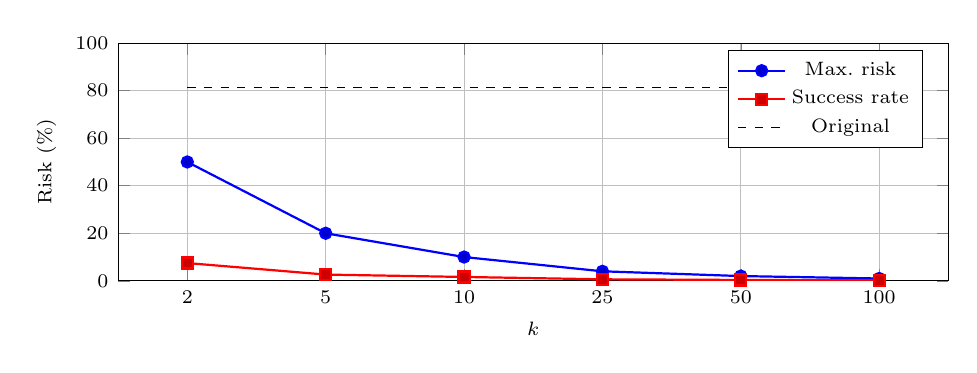
\begin{tikzpicture}
\begin{axis}[width=\textwidth,height=4.6cm,
  symbolic x coords={2,5,10,25,50,100},xtick=data,
  xlabel={$k$},ylabel={Risk (\%)},ymin=0,ymax=100,
  legend style={font=\scriptsize,at={(0.97,0.97)},anchor=north east},
  tick label style={font=\scriptsize},label style={font=\scriptsize},grid=major]
\addplot+[mark=*,thick] coordinates {(2,50)(5,20)(10,10)(25,4)(50,2)(100,0.97)};
\addplot+[mark=square*,thick] coordinates {(2,7.47)(5,2.62)(10,1.62)(25,0.63)(50,0.36)(100,0.19)};
\addplot+[dashed,no marks,black] coordinates {(2,81.5)(100,81.5)};
\legend{Max.\ risk,Success rate,Original}
\end{axis}
\end{tikzpicture}
\caption{Risk vs $k$}
\end{subfigure}\hfill
\begin{subfigure}{0.49\textwidth}
\centering
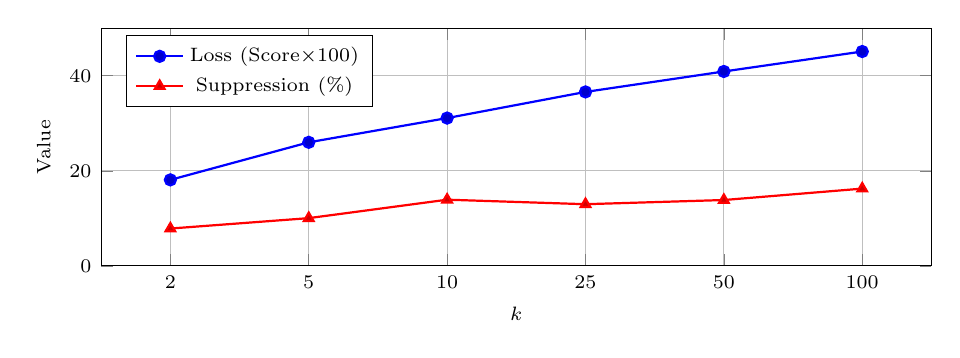
\begin{tikzpicture}
\begin{axis}[width=\textwidth,height=4.6cm,
  symbolic x coords={2,5,10,25,50,100},xtick=data,
  xlabel={$k$},ylabel={Value},ymin=0,ymax=50,
  legend style={font=\scriptsize,at={(0.03,0.97)},anchor=north west},
  tick label style={font=\scriptsize},label style={font=\scriptsize},grid=major]
\addplot+[mark=*,thick] coordinates {(2,18.1)(5,26)(10,31.1)(25,36.6)(50,40.9)(100,45.1)};
\addplot+[mark=triangle*,thick] coordinates {(2,7.86)(5,10.05)(10,13.93)(25,12.98)(50,13.86)(100,16.26)};
\legend{Loss (Score$\times$100),Suppression (\%)}
\end{axis}
\end{tikzpicture}
\caption{Utility vs $k$}
\end{subfigure}

\begin{subfigure}{0.55\textwidth}
\centering
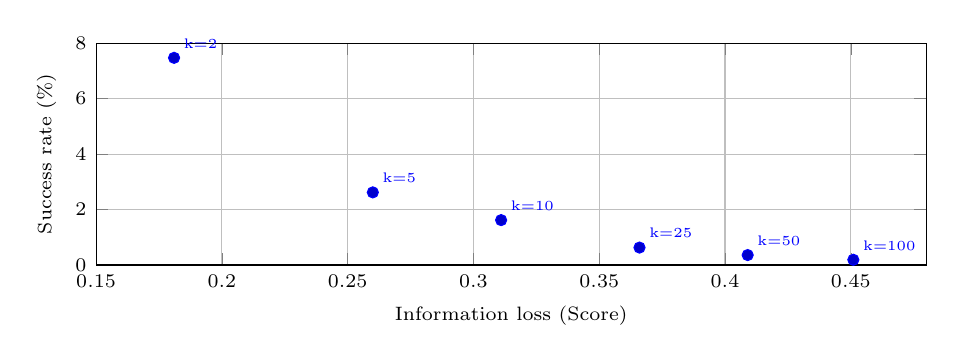
\begin{tikzpicture}
\begin{axis}[width=\textwidth,height=4.4cm,
  xlabel={Information loss (Score)},ylabel={Success rate (\%)},
  xmin=0.15,xmax=0.48,ymin=0,ymax=8,
  tick label style={font=\scriptsize},label style={font=\scriptsize},
  grid=major,nodes near coords,
  point meta=explicit symbolic,
  every node near coord/.append style={font=\tiny,anchor=south west}]
\addplot+[only marks,mark=*] coordinates {
  (0.181,7.47)[k=2] (0.260,2.62)[k=5] (0.311,1.62)[k=10]
  (0.366,0.63)[k=25] (0.409,0.36)[k=50] (0.451,0.19)[k=100]};
\end{axis}
\end{tikzpicture}
\caption{Risk--utility trade-off (frontier)}
\end{subfigure}
\caption{Risk and utility of the \textit{k}-anonymity model as a function of $k$. The maximum risk follows
$1/k$; utility degrades monotonically.}
\label{fig:plots}
\end{figure}

\textbf{Analysis.} Risk decreases predictably: the maximum risk follows $1/k$ (50\%, 20\%, 10\%, 4\%, 2\%,
$\sim$1\%) and the \textit{success rate} drops from 7{,}47\% to 0{,}19\%. Even $k=2$ drastically reduces risk
relative to the original's 81{,}5\%. In contrast, information loss grows monotonically (0{,}18~$\to$~0{,}45).
Notably, \textbf{suppression is not strictly monotonic} ($k=25$ suppresses 12{,}98\%, less than the 13{,}93\% of
$k=10$): by generalizing one attribute more aggressively (e.g.\ raising \textit{age} from level 3 to 4), ARX
reduces the need to suppress records, illustrating the internal trade-off between generalization and
suppression. The \textbf{``knee'' of the curve} lies at $k=5$--$10$, where low risk ($\leq 10\%$) is already
achieved with still-moderate loss; beyond $k=25$ the privacy gain is marginal but the utility cost is high.

\subsection{Model 2: \textit{k}-anonymity + $\ell$-diversity}
We added $\ell$-diversity (\textit{distinct}) over the sensitive attribute \textit{income}, keeping $k=5$. Since
\textit{income} is binary, $\ell=2$ is the \textbf{maximum possible}: an inherent limitation of the
attribute, not a configuration choice, so an $\ell$ sweep is not meaningful. $\ell$-diversity was not applied to
\textit{capital-gain}/\textit{capital-loss}: both have an extremely skewed distribution ($>$91\% zero values),
which makes \textit{distinct} $\ell$-diversity inadequate: a class with \{0,\,0,\,0,\,X\} satisfies $\ell=2$
but offers no real protection against inference. Table~\ref{tab:m2} compares the two models at $k=5$.

\begin{table}[h]
\centering\footnotesize
\begin{tabular}{l c c l}
\toprule
\textbf{Metric} & \textbf{Model 1 ($k{=}5$)} & \textbf{Model 2 ($k{=}5,\ell{=}2$)} & \textbf{Effect of $\ell$-diversity} \\
\midrule
Maximum risk (\%)      & 20{,}0  & 20{,}0  & unchanged ($k$ controls re-identification) \\
Success rate (\%)      & 2{,}62  & 1{,}22  & lower ($-$53\%) \\
Avg.\ class size       & 38{,}23 & 81{,}94 & more aggregated classes \\
Min.\ class size       & 5       & 5       & unchanged \\
Suppression (\%)       & 10{,}05 & 10{,}41 & slightly higher \\
Loss (Score)           & 0{,}260 & 0{,}345 & higher ($+$33\%) \\
\bottomrule
\end{tabular}
\caption{Comparison of pure \textit{k}-anonymity with \textit{k}-anonymity\,+\,$\ell$-diversity ($k=5$).}
\label{tab:m2}
\end{table}

\textbf{Analysis.} $\ell$-diversity \textbf{does not change the re-identification risk} (maximum risk stays at
20\%, controlled by $k$), but it adds protection against a distinct attack vector - \textbf{sensitive
attribute inference}: by requiring each equivalence class to contain both values of \textit{income}, it prevents
the attacker from deducing an individual's income even without identifying them. The cost is higher information
loss ($+$33\%) and larger classes (38~$\to$~82), since the additional constraint forces more generalization
(\textit{age} rises to level 4 and \textit{marital-status} to level 3, which remained at 0 in Model~1). The
\textit{success rate} also drops, but as a side effect of the increased class size.

\subsection{Generalization vs suppression}
The optimal transformation vectors show that ARX favors generalizing \textit{age} and \textit{hours-per-week}
(attributes with deep hierarchies), keeping \textit{marital-status} and \textit{sex} ungeneralized for low $k$.
Suppression acts as a complementary mechanism to eliminate the \textit{outliers} that would otherwise force the
generalization of an entire column, hence the non-monotonic relationship observed in Table~\ref{tab:m1}.

To isolate this trade-off, we performed a dedicated sweep of the \textbf{suppression limit} with $k=5$ fixed
(pure \textit{k}-anonymity), testing the values $\{0, 2, 5, 10, 100\}\%$. Table~\ref{tab:supp} and
Figure~\ref{fig:supp} present the results.

\begin{table}[h]
\centering\footnotesize
\begin{tabular}{c c c c c c}
\toprule
\textbf{Suppr.\ limit (\%)} & \textbf{Max.\ risk (\%)} & \textbf{Success rate (\%)} & \textbf{Min.\ class} & \textbf{Records suppr.\ (\%)} & \textbf{Loss (Score)} \\
\midrule
0   & 7{,}14 & 0{,}15 & 14 & 0{,}00  & 0{,}346 \\
2   & 20{,}0 & 1{,}35 & 5  & 1{,}70  & 0{,}282 \\
5   & 20{,}0 & 1{,}87 & 5  & 4{,}99  & 0{,}264 \\
10  & 20{,}0 & 2{,}39 & 5  & 7{,}50  & 0{,}262 \\
100 & 20{,}0 & 2{,}62 & 5  & 10{,}05 & 0{,}261 \\
\bottomrule
\end{tabular}
\caption{Suppression-limit sweep with $k=5$ fixed. The 0\% case cannot suppress any record and is forced to
over-generalize.}
\label{tab:supp}
\end{table}

\begin{figure}[h]
\centering
\begin{subfigure}{0.49\textwidth}
\centering
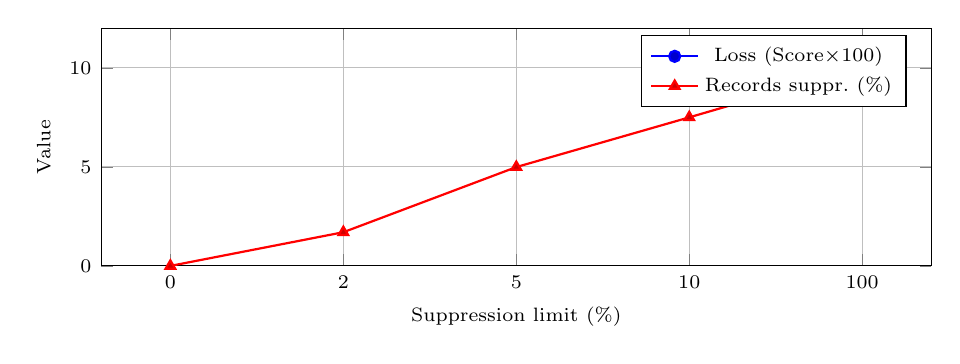
\begin{tikzpicture}
\begin{axis}[width=\textwidth,height=4.6cm,
  symbolic x coords={0,2,5,10,100},xtick=data,
  xlabel={Suppression limit (\%)},ylabel={Value},ymin=0,ymax=12,
  legend style={font=\scriptsize,at={(0.97,0.97)},anchor=north east},
  tick label style={font=\scriptsize},label style={font=\scriptsize},grid=major]
\addplot+[mark=*,thick] coordinates {(0,34.6)(2,28.2)(5,26.4)(10,26.2)(100,26.1)};
\addplot+[mark=triangle*,thick] coordinates {(0,0)(2,1.70)(5,4.99)(10,7.50)(100,10.05)};
\legend{Loss (Score$\times$100),Records suppr.\ (\%)}
\end{axis}
\end{tikzpicture}
\caption{Information loss vs records suppressed}
\end{subfigure}\hfill
\begin{subfigure}{0.49\textwidth}
\centering
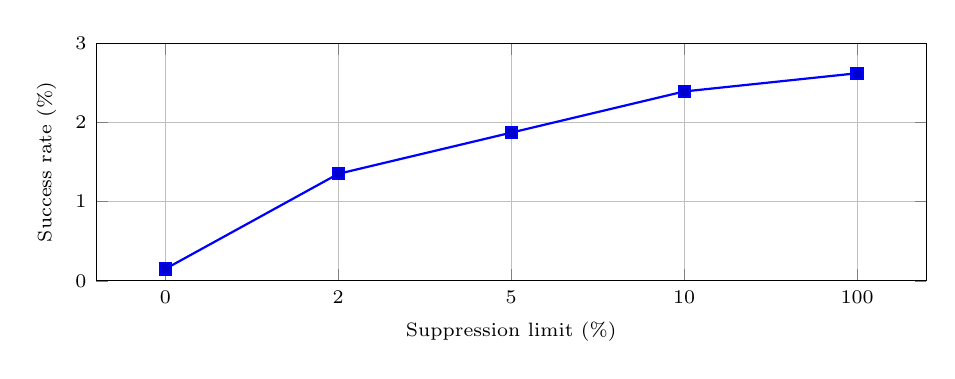
\begin{tikzpicture}
\begin{axis}[width=\textwidth,height=4.6cm,
  symbolic x coords={0,2,5,10,100},xtick=data,
  xlabel={Suppression limit (\%)},ylabel={Success rate (\%)},ymin=0,ymax=3,
  tick label style={font=\scriptsize},label style={font=\scriptsize},grid=major]
\addplot+[mark=square*,thick] coordinates {(0,0.15)(2,1.35)(5,1.87)(10,2.39)(100,2.62)};
\end{axis}
\end{tikzpicture}
\caption{Residual risk (success rate)}
\end{subfigure}
\caption{Effect of the suppression limit at $k=5$. Allowing more suppression lowers generalization-driven
information loss but raises both the suppression count and the residual risk, until both plateau near the
$\sim$10\% the optimal solution naturally requires.}
\label{fig:supp}
\end{figure}

\textbf{Analysis.} The sweep cleanly exposes the generalization\,/\,suppression trade-off. The
\textbf{$0\%$ case is the most revealing}: forbidden from suppressing any record, ARX must generalize until
\emph{every} class (including outliers) reaches $k=5$, producing the deepest transformation
($[3,1,2,1,1,1,0,3,2]$), the highest information loss (0{,}346), and --- as a side effect --- an average class
size of 678 and a maximum risk of only \textbf{7{,}14\%} (well below the requested 20\%, since the minimum class
ends up at 14). As the suppression limit increases, ARX trades generalization for the removal of those outliers:
information loss drops (0{,}346~$\to$~0{,}261) while suppressed records rise (0\%~$\to$~10{,}05\%) and the
residual risk climbs toward the $1/k=20\%$ ceiling. Both curves \textbf{plateau beyond $\sim$10\%}, because the
optimal solution never needs to suppress more than the 10{,}05\% it requires at the 100\% limit --- so limits of
10\% and 100\% yield virtually identical results. The best balance lies around a \textbf{2--5\% limit}, which
recovers most of the utility lost at 0\% while suppressing only a small fraction of records.

% ==================================================================
\section{Iterations and Recommended Configuration}
% ==================================================================
The $k$ sweep, the suppression-limit sweep, and the introduction of $\ell$-diversity constitute the planned
refinement iterations: the first identifies the risk/utility equilibrium point, the second tunes the
generalization/suppression balance, and the third adds protection against inference at a utility cost.
As an additional refinement, \textbf{local transformation} (instead of global) could improve utility by allowing
distinct generalization levels per group of records, a direction to explore in future work.
\textbf{Recommended configuration:} for a balanced risk/utility trade-off, $k=5$ to $k=10$ with a suppression
limit of about 2--5\% (which recovers most of the utility while suppressing few records); if protection against
\textit{income} inference is a requirement, $k=5$\,+\,$\ell=2$.

% ==================================================================
\section{Conclusion}
% ==================================================================
Anonymization reduced the re-identification risk drastically: the \textit{success rate} fell from 81{,}5\%
(original) to 2{,}62\% ($k=5$) and the worst case from 100\% to 20\%, with 0\% of records at high risk. The
utility cost is controlled and grows with $k$. $\ell$-diversity complements $k$-anonymity by covering a
different attack vector. The risk/utility trade-off confirms $k=5$--$10$ as the best-balance region for this
dataset.

% ==================================================================
\section*{Documentation of AI Use}
% ==================================================================
\small
During the development of this work, an AI assistant (Claude, Anthropic) was used as support, under the group's
review and validation, for the following tasks: (i) planning the ARX workflow; (ii) guidance on building the
generalization hierarchies (level structure and groupings); (iii) computing supporting statistics for the
classification and \textit{coding model} decisions (distinction/separation values, distribution of attributes
such as \textit{age}, \textit{hours-per-week}, \textit{race}, and empirical validation of the \texttt{South}
disambiguation); (iv) organizing the metrics collected in ARX into a spreadsheet and generating the plots;
(v) support in drafting and structuring this report. All anonymization runs, metric collection, and final
decisions were carried out and verified by the authors in the ARX tool.

\end{document}